\author{João Gonçalves}
\newcommand{\authorD}{Daniel Dinis}
\newcommand{\authorM}{Martim Bento}
\newcommand{\authorT}{Tiago Brogueira}
\newcommand{\studentID}{99995}
\newcommand{\studentIDD}{99906}
\newcommand{\studentIDM}{100031}
\newcommand{\studentIDT}{100095}
\newcommand{\supervisorone}{Prof\textsuperscript{\underline{a}}. Célia Jesus}
\newcommand{\supervisortwo}{}
\newcommand{\department}{Engenharia Eletrotécnica e de Computadores}
\newcommand{\exam}{Electrotecnia Teórica}

\title{%
3\textsuperscript{\underline{o}} Trabalho Laboratorial\\
\large CIRCUITO RLC-SÉRIE\\
\big (em Regime Forçado Alternado Sinusoidal)}
\date{Abril 2022}

\documentclass[a4paper,12pt]{article}
\usepackage[left=30mm,top=30mm,right=30mm,bottom=30mm]{geometry}
\usepackage{etoolbox}
\usepackage{pgfplots}
\usepackage{circuitikz}
\usepackage{booktabs}
\usepackage[usestackEOL]{stackengine}
\usepackage[T1]{fontenc}
\usepackage[utf8]{inputenc}
\usepackage{bm}
\usepackage[export]{adjustbox}
\usepackage{graphicx}
\usepackage{subcaption}
\usepackage{amsmath}
\usepackage{amsfonts}
\usepackage{mathtools}
%\usepackage[svgnames]{xcolor}
\usepackage{float}
\usepackage{hyperref}
\usepackage[capitalise]{cleveref}
\usepackage{enumitem,kantlipsum}
\usepackage[square,numbers,sort]{natbib}
\usepackage[ruled,vlined]{algorithm2e}
\usepackage{listings}
\usepackage{minted}
\usepackage{amssymb}
\usepackage{babel}
\usemintedstyle{emacs}
%\setlength{\parindent}{0pt}

\renewcommand{\listingscaption}{Algorithm}
\renewcommand{\listoflistingscaption}{List of Algorithms}
\renewcommand{\figurename}{Fig.}
\renewcommand{\tablename}{Tab.}
\renewcommand{\contentsname}{Índice}

\bibliographystyle{unsrtnat}

\hypersetup{
    colorlinks,
    linkcolor={black},
    citecolor={blue!50!black},
    urlcolor={blue!80!black}
}

\linespread{1}

\newtheorem{theorem}{Theorem}[section]
\graphicspath{{figures/}}	

%----------------------------------TITLE PAGE -----------------------------------
\makeatletter
\def\maketitle{
  \begin{center}\leavevmode
       \normalfont
       
\includegraphics[width=0.55\columnwidth]{IST.pdf}
       \vskip 1.5cm   
       \textsc{\large \department}\\
       \vskip 1.5cm
       \rule{\linewidth}{0.2 mm} %\\
       {\large \exam}\\[1 cm]
       {\huge \bfseries \@title \par}
       \vspace{1cm}
	\rule{\linewidth}{0.2 mm} \\[1.5 cm]
	 
	\begin{minipage}[t]{0.45\textwidth}
		\begin{flushleft} \large
			\emph{Autores:}\\
            \textbf{\authorD} : \studentIDD\\
			\textbf{\@author} : \studentID\\
            \textbf{\authorM} : \studentIDM\\
			\textbf{\authorT} : \studentIDT
		\end{flushleft}
	\end{minipage}
	\begin{minipage}[t]{0.45\textwidth}
	   \begin{flushright} \large
			\ifdefempty{\supervisortwo}{\emph{Supervisora:\\}}{\emph{Supervisores:\\}}
			\supervisorone\\
			\ifdefempty{\supervisortwo}{}{\supervisortwo\\}
		\end{flushright}
	\end{minipage}
	\vfill
	{\Large \@date\par}
   \end{center}
   %\vfill
   %\null
   \cleardoublepage
  }
\makeatother
%-------------------------------- ENDTITLE PAGE ----------------------------------

\pgfplotsset{compat=1.18}
\begin{document}

\pagenumbering{gobble}
\maketitle
\newpage
\pagenumbering{arabic}

\section*{Questões}
%\clearpage
%//==============================--@--==============================//%
\subsection*{\underline{3.1} Verifique que o factor de qualidade $Q_0$ num circuito RLC-série é a sobretensão de $U_{Lef}$ ou $U_{Cef}$ em relação à tensão aplicada $U_{Gef}$ na situação de ressonância.}
\paragraph{Resposta:}
O factor de qualidade $Q_0$  é uma característica de um circuito ressonante (como é o caso do circuito RLC-série) que mede a qualidade dos componentes reactivos. Este factor indica-nos a relação entre a energia armazenada e a energia dissipada:

$$ Q_0 = 2\pi \cdot \frac{\text{(Energia máxima armazenada)}}{\text{(Energia perdida p/ ciclo)}} $$

Note-se que as perdas de energia por ciclo nada mais são do que a potência média dissipada por período, i.e., temos:

$$ Q_0 = 2\pi \cdot \frac{\text{(Energia máxima armazenada)}}{\text{(Potência média dissipada)}\cdot T_0} = \omega_0 \cdot \frac{\text{(Energia máxima armazenada)}}{\text{(Potência média dissipada)}}$$

Do Teorema de Poynting complexo é-nos trivial deduzir que no estado de ressonância, a potência reactiva é \underline{nula}. Isto indica que tanto a bobina como o condensador estão a produzir a mesma energia, mas como estão em oposição de fase, anulam-se. Sendo assim, olhamos para o circuito como puramente resistivo. (Observa-se que $\vert \bar{Z}_{eq}\vert = R \land \vert \bar{I}\vert = \vert\bar{I}\vert_{MAX} = \frac{U_{G}}{R}$).

$$ 
\implies Q_0 = \omega_o \frac{(W_m)_{MAX}}{(p_J)_{av}} = \omega_0 \frac{\frac{1}{2}LI_{ef}^2}{R\ (\frac{I_{ef}}{\sqrt{2}})^2} = \frac{\omega_0 L}{R}\\ 
$$

$$
\implies Q_0 = \omega_o \frac{(W_e)_{MAX}}{(p_J)_{av}} = \omega_0 \frac{\frac{1}{2}C U_{ef}^2}{R\ (\frac{I_{ef}}{\sqrt{2}})^2} = \omega_0 \frac{\frac{1}{2} C I_{ef}^2 \mathcal{X}_c^2}{\frac{1}{2}I_{ef}^2\ R} = \frac{1}{\omega_0 RC}\ \text{, com}\ \mathcal{X}_c = \frac{1}{\omega_0 C}
$$

$$
\therefore Q_0 = \frac{\omega_0 L}{R} = \frac{1}{\omega_0 RC} = \frac{1}{R}\sqrt{\frac{L}{C}}
$$
\hfill \ensuremath{\Box}

No estado de ressonância as tensões no condensador e na bobina são de igual amplitude.

$$
\begin{dcases*}
U_L = I \mathcal{X}_L = I\cdot \omega_0 L = \frac{\omega_0 L}{R}\cdot U_G = Q_0\cdot U_G\\
U_C = I \mathcal{X}_C = \frac{I}{\omega_0 C} = \frac{1}{\omega_0 RC}\cdot U_G = Q_0\cdot U_G
\end{dcases*}
$$

Trivialmente concluímos que em ressonância: 
$$ 
Q_0 = \dfrac{U_L}{U_G} = \dfrac{U_C}{U_G} \iff Q_0 = \dfrac{U_{Lef}}{U_{Gef}} = \dfrac{U_{Cef}}{U_{Gef}}
$$
\hfill \ensuremath{\Box}
%//==============================--@--==============================//%
\clearpage
%//==============================--@--==============================//%
\subsection*{\underline{3.2} Considere o circuito RLC-série, com frequência de ressonância $\mathbf{f_0 = 60}\ \text{kHz}$ e admita que o valor estimado do coeficiente de auto-indução da bobina é $\mathbf{L = 3.0}\ \text{mH}$.}
%//==============================--A--==============================//%
\subsubsection*{(a) Determine o valor da capacidade C tal que o circuito esteja em ressonância à frequência $f_0$ indicada.}
\label{subsubsec_a}
\paragraph{Resposta:}
De acordo com as derivações e conclusões da alínea anterior, podemos imediatamente verificar que $\omega_0 L = \dfrac{1}{\omega_0 C}$. Pelo que, naturalmente, concluímos a expressão em ordem à incógnita:

$$
C = \frac{1}{\omega_0^2 L} \approx 2.345\ \text{nF}
$$

%//==============================--B--==============================//%
\subsubsection*{(b) Trace duas curvas da corrente normalizada, $I_n$, em função da frequência normalizada. Para cada um dos valores de $R=R_S$, determine as frequências das situações de meia potência $f_1$ e $f_2$, e determine, para cada caso, a largura de banda em valores absolutos $\Delta f$. Verifique (10).}
\paragraph{Resposta:}
Tendo em conta a frequência de ressonância $f_0 = 60\ \text{kHz}$ e o intervalo de frequências a que nos restringimos, i.e., $f \in \left[20; 90\right]\ \text{kHz}$, segue-se que a frequência normalizada ($f_n = \dfrac{f}{f_0}$) é delimitada no seguinte
intervalo: $f_n \in \left[\frac{1}{3}; \frac{3}{2}\right]$. 

\def\varQR{(2*pi*1.8)^2}
\def\varQRR{(2*pi*0.45)^2}
\def\fnum{-1/(2*2*pi*1.8)+sqrt(1/(4*(2*pi*1.8)^2)+1)}
\def\fndois{1/(2*2*pi*1.8)+sqrt(1/(4*(2*pi*1.8)^2)+1)}
\def\fntres{-1/(2*2*pi*0.45)+sqrt(1/(4*(2*pi*0.45)^2)+1)}
\def\fnquatro{1/(2*2*pi*0.45)+sqrt(1/(4*(2*pi*0.45)^2)+1)}
\begin{figure}[!h]  
    \begin{subfigure}[b]{0.45\textwidth}
    \centering
    \resizebox{1\textwidth}{!}{%
        \begin{tikzpicture}
            \begin{axis}[
                axis lines = left,
                xlabel = {Frequência normalizada ($f_n$)},
                ylabel = {Corrente normalizada ($I_n$)},
                grid style=dashed,
                grid=major
            ]

            \addplot [
                domain=(1/3):(3/2), 
                samples=300, 
                color=red,
            ]
            { 1/sqrt( 1/(\varQR) + (x-1/x)^2 )};
            
            \addplot[
                domain=(1/3):(3/2), 
                samples=300, 
                color=magenta,
                dashed
            ]
            {2*pi*1.8/sqrt(2)};
            
            \addplot [only marks,mark=*,dashed,color=magenta] coordinates { (\fnum,2*pi*1.8/sqrt(2)} \node[pin=150:{$f_{n1}$}]{} ;
            
            \addplot [only marks,mark=*,dashed,color=magenta] coordinates { (\fndois,2*pi*1.8/sqrt(2)};
            
            \addplot +[mark=none,color=magenta,dashed] coordinates {(\fnum, 0.5) (\fnum, 2*pi*1.8/sqrt(2))};
            
            \addplot +[mark=none,color=magenta,dashed] coordinates {(\fndois, 0.5) (\fndois, 2*pi*1.8/sqrt(2))};
            
            %\addlegendentry{}
            \end{axis}
        \end{tikzpicture}
    }%
    \caption{Caso com $R=R_S=100\ \Omega$}
    \end{subfigure}
    \hfill
    \begin{subfigure}[b]{0.45\textwidth}
    \centering
    \resizebox{1\textwidth}{!}{%
        \begin{tikzpicture}
            \begin{axis}[
                axis lines = left,
                xlabel = {Frequência normalizada ($f_n$)},
                ylabel = {Corrente normalizada ($I_n$)},
                grid style=dashed,
                grid=major
            ]

            \addplot [
                domain=(1/3):(3/2), 
                samples=300, 
                color=blue,
            ]
            { 1/sqrt( 1/(\varQRR) + (x-1/x)^2 )};
            
            \addplot[
                domain=(1/3):(3/2), 
                samples=300, 
                color=cyan,
                dashed
            ]
            {2*pi*0.45/sqrt(2)};
            
            \addplot [only marks,mark=*,dashed,color=cyan] coordinates { (\fntres,2*pi*0.45/sqrt(2)};
            
            \addplot [only marks,mark=*,dashed,color=cyan] coordinates { (\fnquatro,2*pi*0.45/sqrt(2)};
            
            \addplot +[mark=none,color=cyan,dashed] coordinates {(\fntres, 0.3) (\fntres, 2*pi*0.45/sqrt(2))};
            
            \addplot +[mark=none,color=cyan,dashed] coordinates {(\fnquatro, 0.3) (\fnquatro, 2*pi*0.45/sqrt(2))};
            %\addlegendentry{}
            \end{axis}
        \end{tikzpicture}
    }%
    \caption{Caso com $R=R_S=400\ \Omega$}
    \end{subfigure}
\caption{Curvas de corrente normalizada para os dois valores possíveis da resistência (com os respectivos pontos de meia potência normalizados).} \label{fig:curvas_ressonancia} 
\end{figure}

$$
R=100\ \Omega:
\begin{cases}
    f_{n1} = 0.956757\\
    f_{n2} = 1.045186
\end{cases}
\implies \Delta f_n = 0.088419 \implies \Delta f = 5305\ \text{Hz}
$$

$$
R=400\ \Omega:
\begin{cases}
    f_{n1} = 0.838677\\
    f_{n2} = 1.192354
\end{cases}
\implies \Delta f_n = 0.353678 \implies \Delta f = 21220\ \text{Hz}
$$

$$
R=100\ \Omega:
\begin{cases}
    Q_0 = 11.309734\\
    \Delta f_n = 0.088419
\end{cases}
\land\
R=400\ \Omega:
\begin{cases}
    Q_0 = 2.827433\\
    \Delta f_n = 0.353678
\end{cases}
$$

Pelo que, naturalmente se verifica a relação enunciada $\Delta f_n = \dfrac{1}{Q_0}$.

$$
R=100\ \Omega:
\begin{cases}
    \dfrac{1}{Q_0} = 0.088419\\
    \Delta f_n = 0.088419
\end{cases}
\land\
R=400\ \Omega:
\begin{cases}
    \dfrac{1}{Q_0} = 0.353678\\
    \Delta f_n = 0.353678
\end{cases}
$$

$$\therefore \Delta f_n = \frac{1}{Q_0}$$
\hfill \ensuremath{\Box}
%//==============================--C--==============================//%
\subsubsection*{(c) Para o caso $R_S = 100\ \Omega$, $U_{gef} = 1\ \text{V}$ e tomando $C$ o valor determinado em \hyperref[subsubsec_a]{(a)}, calcule os valores eficazes e desfasagens da corrente $i$ e das tensões no condensador, $u_C$, na bobina, $u_L$, e na resistência, $u_R$, para a frequência de ressonância, $f_0$, bem como para as frequências $f_1$ e $f_2$.}
%//==============================--D--==============================//%
\subsubsection*{(d) Para as condições da alínea anterior e para cada uma dessas três frequências trace os correspondentes diagramas vectoriais de tensão.}
%//==============================--@--==============================//%
\clearpage
%//==============================--@--==============================//%
\subsection*{\underline{3.3} Demonstre as expressões (11) e (12).}
\paragraph{Resposta:}
Para simplificar a análise do novo circuito, queremos converter a malha numa impedância equivalente, $Z'$, como ilustrado na \hyperref[fig:ideia]{Fig. 3}. Após tal tarefa, torna-se trivial a análise, visto que se torna num circuito em série que se assemelha ao anteriormente estudado.

\iffalse
\begin{figure}[H]
    \centering
    \includegraphics[width = 0.5\linewidth]{unknown.png}
    \caption{Estratégia para simplificação da malha.}
    \label{fig:ideia}
\end{figure}
\fi

\begin{figure}[htb]%
    \centering
    \begin{circuitikz} \draw
        (0,0) to[open,o-] (0,0) to (1,0) to[R, l=$R_L$] (3,0) to[L, l=$L$] (5,0) to (6,0) to[open,-o] (6,0)
        (1,0) to (1,-1) to (2,-1) to[C, l=$C_d$] (4,-1) to (5,-1) to (5,0) 
    ;
    \end{circuitikz}
    \qquad
    \subfloat{{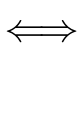
\includegraphics[scale=0.4,valign=t]{teste.png} }}%
    \qquad
    \begin{circuitikz} \draw
        (0,1) to[open,o-] (0,1) to (1,1) to[fullgeneric, l=$Z'$] (2,1) to (3,1) to[open,-o] (3,1)
        (0,0)
    ;
    \end{circuitikz}
    \caption{Estratégia para simplificação da malha.}
    \label{fig:ideia}
\end{figure}

\begin{equation}
    \label{eq2}
    \begin{cases}
        \overrightarrow{\nabla} \cdot \overrightarrow{J} \approx 0\\
        \overrightarrow{\nabla} \times \overrightarrow{E} = -\dfrac{\partial}{\partial t}\overrightarrow{B}
    \end{cases}
    \implies
    \begin{cases}
        \bar{I} = \bar{I}_{1} + \bar{I}_{2}\\
        \bar{U}_{1} = \bar{U}_{2} = \bar{U}_{malha}
    \end{cases}
\end{equation}

$$
    \begin{cases}
        \bar{I}_1 = \dfrac{1}{R_L + j\omega L}\ \bar{U}_1\\
        \bar{I}_2 = \dfrac{1}{1/(j\omega C_d)}\ \bar{U}_2
    \end{cases}
    \xRightarrow[]{\hyperref[eq2]{(2)}}
    \bar{I} = (\frac{1}{R_L + j\omega L} + \frac{1}{1/(j\omega C_d)})\bar{U}_{malha} 
$$

Aplicando a Lei de Ohm facilmente obtemos $\bar{Z}'$, i.e.:

$$
    \bar{Z}' = \frac{\bar{U}_{malha}}{\bar{I}} = \frac{(R_L + j\omega L)[1/(j\omega C_d)]}{R_L + j\omega L + [1/(j\omega C_d)]}
$$

De acordo com o plano, agora podemos analizar em conformidade com o conceito de circuito em série:

$$
\bar{U}_G = \bar{U}_R + \bar{U}_{malha} + \bar{U}_C \implies \bar{U}_G = (R_S + \frac{(R_L + j\omega L)[1/(j\omega C_d)]}{R_L + j\omega L + [1/(j\omega C_d)]} + \frac{1}{j\omega C})\ \bar{I}
$$

$$
\therefore \bar{Z}_{eq} = \frac{\bar{U}_G}{\bar{I}} = R_S + \frac{1}{j\omega C} + \frac{(R_L + j\omega L)[1/(j\omega C_d)]}{R_L + j\omega L + [1/(j\omega C_d)]}
$$
\hfill \ensuremath{\Box}

Supondo $R_L << \omega L$, temos que $R_L + j\omega L \approx j\omega L$, e assim obtemos a seguinte aproximação:

$$
\bar{Z}_{eq} = R_S + \frac{1}{j\omega C} + \frac{(j\omega L)[1/(j\omega C_d)]}{j\omega L + [1/(j\omega C_d)]} = R_S - j(\frac{1}{\omega C} + \frac{\omega L}{\omega^2 L C_d - 1})
$$

Para deduzir a nova frequência de ressonância, basta ter em consideração que o circuito durante o fenómeno é puramente resistivo, i.e., $\mathbb{I}m\{\bar{Z}_{eq}\} = 0$.

$$
\mathbb{I}m\{\bar{Z}_{eq}\} = 0
\implies
\frac{1}{\omega C} + \frac{\omega L}{\omega^2 L C_d - 1} = 0
\iff
\frac{1-\omega^2 L C_d}{\omega C(1-\omega^2 L C_d)} = \frac{\omega^2 L C}{\omega C(1-\omega^2 L C_d)}
$$

Por conseguinte, temos que a relação $1 = \omega^2 L C_d + \omega^2 L C$ deve ser satisfeita para dado $\omega$, de modo a que se verifique um estado de ressonância no novo circuito (note-se que o denominador não se anula, evitando a singularidade).

$$
    \therefore \frac{1}{\omega^2} = L(C + C_d)
$$
\hfill \ensuremath{\Box}
%//==============================--@--==============================//%}


\end{document}
